\chapter{Propozycja systemu}
\label{cha:propozycja-systemu}

Na Rysunku \ref{fig:system-architecture} przedstawiono system automatyki domowej, którego projekt i implementacja leżą w zakresie kolejnych rozdziałów.

\begin{figure}[H]
    \centering
    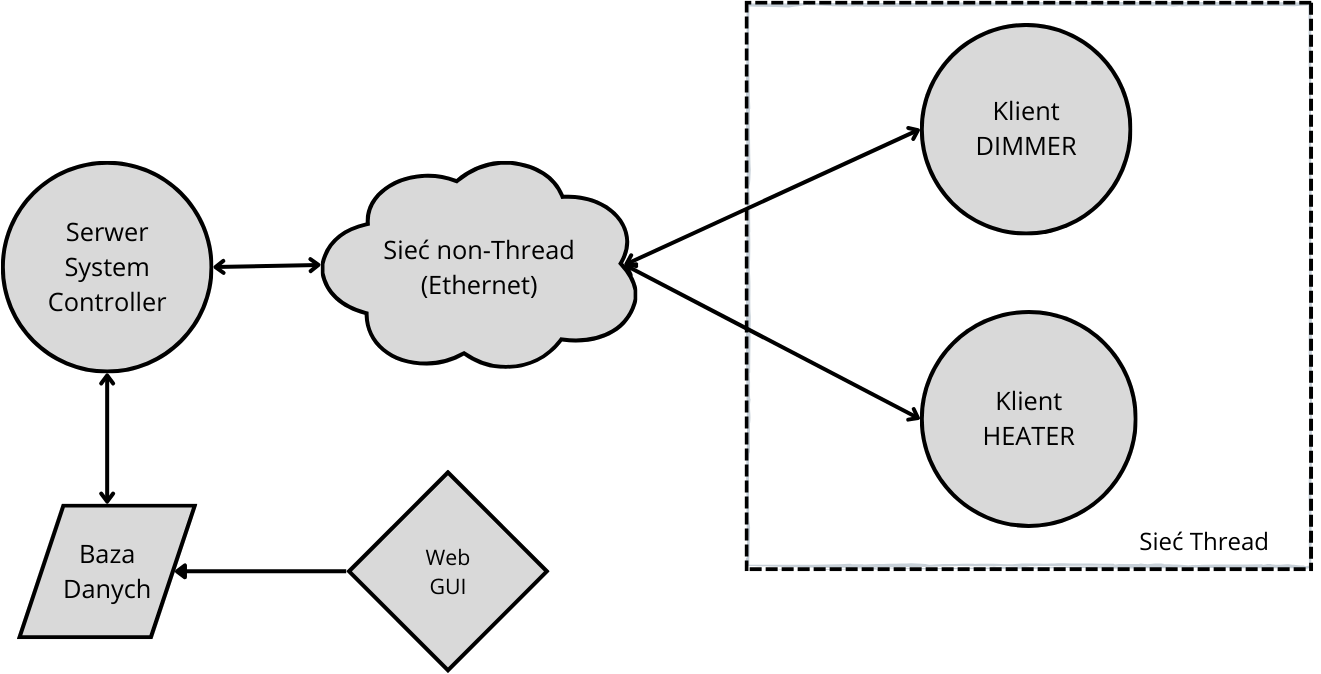
\includegraphics[width=0.8\linewidth]{graphics/system-architecture.png}
    \caption{Proponowana architektura systemu automatyki domowej.}
    \label{fig:system-architecture}
\end{figure}

W dalszej części pracy termin \textit{parametr regulacji}, będzie odnosił się do procentowego stosunku aktualnej mocy układu regulacji do jego maksymalnej wartości mocy.

Funkcją systemu jest utrzymanie zdefiniowanych w Tabeli \ref{tab:profiles-parameters} parametrów środowiska, na poziomie zadanym przez użytkownika systemu. W tym celu urządzenia systemu dokonują pomiaru parametrów oraz regulacji swojej mocy.

\begin{table}[H]
    \centering
    \caption{Zestaw parametrów określonych dla zdefiniowanych profili.}
    \begin{tabular}{|c|c|c|}
         \hline
         \rowcolor{gray!20}
          & HEATER & DIMMER \\
         \hline
         \cellcolor{gray!20}Parametr & temperatura & natężenie oświetlenia \\
         \hline
         \cellcolor{gray!20}Jednostka & $^{\circ}$C & lux \\
         \hline
    \end{tabular}
    \label{tab:profiles-parameters}
\end{table}

Zaproponowany system opiera się o architekturę klient-serwer i składa się z 5 funkcjonalnych bloków:
\begin{enumerate}
    \item klienta Dimmer,
    \item klienta Heater,
    \item serwera z aplikacją System Controller,
    \item Bazy Danych,
    \item Web GUI (ang. \textit{Graphical User Interface}).
\end{enumerate}

Celem niniejszego rozdziału jest omówienie zaproponowanego systemu oraz opisanie jego poszczególnych komponentów. 

\section{Strona kliencka}
\label{sec:system-clients}

Klientami w systemie są urządzenia połączone w sieć Thread, realizujące profile określone w Tabeli \ref{tab:profiles-parameters}. Rolą HEATER oraz DIMMER jest implementacja usług pomiaru i regulacji, odpowiednio, temperatury oraz natężenia oświetlenia.
Klienci komunikują się z serwerem w celu dostarczenia pomiarów oraz uzyskania informacji o decyzji dotyczącej konieczności regulacji mocy.
    
\section{Strona serwera}

System Controller to aplikacja znajdująca się w sieci spoza domeny Thread, pełniąca rolę serwera. Komponent przetwarza otrzymane wartości aktualnego stanu środowiska i uwzględniając zadane przez użytkownika wartości, dokonuje decyzji odnośnie regulacji. Ostatecznie aplikacja powiadamia klientów HEATER oraz DIMMER o konieczności zmiany parametru regulacji.

Dodatkowo System Controller odpowiedzialny jest za logowanie otrzymanych wartości aktualnego stanu parametrów oraz podjęte decyzje odnośnie regulacji.

\section{Sterowanie i logowanie}

W celu zadania wartości parametrów, do których powinien dążyć system, użytkownik korzysta z Web GUI. Graficzny interfejs umożliwia zdefiniowanie stanu, jak również wgląd do logów systemu.

Wpisy systemowe oraz zadeklarowany stan parametrów użytkownika, przechowywane są w bazie danych, do której dostęp ma zarówno Web GUI, jak i System Controller.